\section{问题二：变物性热质耦合与全过程输出}
\label{sec:q2}

\begingroup
% Local white-space settings; body fonts, leading and margins are unchanged.
\setlength{\parskip}{0pt}
\setlength{\abovedisplayskip}{4pt}
\setlength{\belowdisplayskip}{4pt}
\setlength{\abovedisplayshortskip}{4pt}
\setlength{\belowdisplayshortskip}{4pt}
\setlength{\intextsep}{6pt}
\setlength{\textfloatsep}{6pt}
\setlength{\floatsep}{6pt}
\captionsetup{skip=5pt}
\renewcommand{\arraystretch}{1.08}
问题二在第\ref{sec:common-model}章统一模型基础上，采用附录3变物性，从共同初态
联立求解固定半径下的径向温湿场。通过温度与含水率对物性的反馈，
给出规定结果及所设环境延拓下的全程轨迹，为问题三判定终点提供基础。
求解流程见图\ref{fig:q2-workflow}。

\begin{figure}[H]
\centering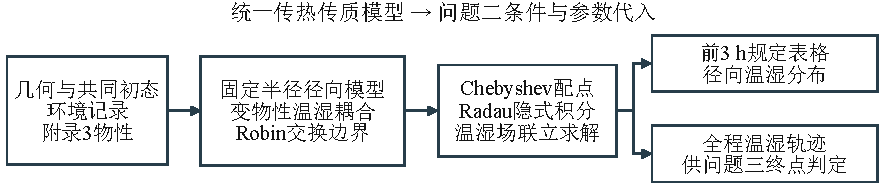
\includegraphics[width=\linewidth]{figures/legibility_schematics/q2_workflow.pdf}
\caption{问题二由统一模型到变物性热质耦合模型的求解流程}
\label{fig:q2-workflow}
\end{figure}

\subsection{从通用方程到变物性耦合系统}
第二问从共同初态开始，全程使用附录3物性，不接续第一问
末态，也不在$1800\unit{s}$处切换公式。有效热容量
$S(C)=\rho_{\rm eff}(C)c_p(C)$和导热率随局部含水率改变，扩散率同时
依赖局部绝对温度$T_K=T+273.15$和$C$。升温改变扩散，失水又通过热容量
及导热率反馈温度，因此需联立推进两个场。

将表\ref{tab:properties}的第二问参数写成
\begin{equation}
\begin{aligned}
S(C)&=(650+128C)\left(1450+\frac{2736C}{1+C}\right),
& k(C)&=0.21+\frac{0.38C}{1+C},\\
D(T,C)&=A(T)e^{-0.45/C},
& A(T)&=2.4\times10^{-3}e^{-3850/T_K}.
\end{aligned}
\label{eq:q2-coefficients}
\end{equation}
固定骨架给出$v_s=0$，空间均匀的参考干密度可从式\eqref{eq:moisture}
约去。再将式\eqref{eq:heat}、\eqref{eq:moisture}的散度取为圆柱径向形式，得
\begin{equation}
\begin{aligned}
T_t&=\frac{1}{rS(C)}\partial_r\!\left[rk(C)T_r\right],\\
C_t&=\frac1r\partial_r\!\left[rA(T)e^{-0.45/C}C_r\right],
\qquad 0<r<R_0.
\end{aligned}
\label{eq:q2-radial}
\end{equation}
例如第一式展开为$T_t=(k/S)(T_{rr}+T_r/r)+(k'(C)/S)C_rT_r$，
显式给出含水率梯度对导热的反馈；不能将其改成
$\nabla\cdot[(k/S)\nabla T]$，否则会额外引入$S$的空间导数。
这里经验$\rho_{\rm eff}(C)$仅用于有效热容量，不同时充当固定体积下
满足真实组成守恒的湿体密度。初态为$T=28\celsius$、$C=2.55$，
轴线零梯度和表面交换沿用式\eqref{eq:boundary}。

\subsection{坐标变换、表面闭合与联合积分}
为避免直接计算$r=0$处的$1/r$，令$x=(r/R_0)^2$。对任意光滑径向场
$v$及系数$a$，由链式法则得到
\begin{equation}
\partial_r=\frac{2r}{R_0^2}\partial_x,\qquad
\frac1r\partial_r(ra\partial_rv)
=\frac4{R_0^2}\partial_x(xa\partial_xv).
\label{eq:q2-coordinate}
\end{equation}
有限的$v_x$自动满足轴线$v_r=0$，且$x=0$处右端取
$4a(0)v_x(0)/R_0^2$，无需人为设置一个很小的替代半径。
按式\eqref{eq:primitive}取$U(C)=\int_0^C e^{-0.45/s}\dd s$，
则$U'(C)=e^{-0.45/C}>0$，水分通量中的$D C_x$恰好等于$A(T)U_x$。
这保留局部温度依赖，并使求导作用于较平缓的原函数场。

在$x_j=[1-\cos(j\pi/N)]/2$，$j=0,\ldots,N$上插值，
记$\mathsf D_x=(\ell'_j(x_i))$为Lagrange插值求导矩阵，
$\mathsf X=\operatorname{diag}(x_j)$；$\mathsf D_x$与物性扩散率$D$含义不同。
对包含表面的节点向量，令
$\boldsymbol q_T=\operatorname{diag}(k_j)\mathsf D_x\boldsymbol T$、
$\boldsymbol q_C=\operatorname{diag}(A_j)\mathsf D_x\boldsymbol U$。
由$\partial_x(xq)=q+xq_x$逐项配点，得到实际采用的半离散系统
\begin{equation}
\begin{aligned}
\dot{\boldsymbol T}_{I}
&=\frac4{R_0^2}
 \left[\operatorname{diag}(S_j^{-1})
 (\mathsf I+\mathsf X\mathsf D_x)\boldsymbol q_T\right]_{I},\\
\dot{\boldsymbol C}_{I}
&=\frac4{R_0^2}
 \left[(\mathsf I+\mathsf X\mathsf D_x)\boldsymbol q_C\right]_{I},
\qquad I=\{0,\ldots,N-1\}.
\end{aligned}
\label{eq:q2-semidscrete}
\end{equation}
其中$\mathsf I$是单位矩阵，下标$I$表示取待积分节点；表面$j=N$
不另设演化方程。由式\eqref{eq:boundary}及$\partial_r=(2/R_0)\partial_x$
在表面联立求解
\begin{equation}
\begin{aligned}
\gamma k(C_s)(\mathsf D_x\boldsymbol T)_N+h_T(T_s-T_a)&=0,\\
\gamma A(T_s)(\mathsf D_x\boldsymbol U)_N+h_m(C_s-b)&=0,
\qquad\gamma=\frac2{R_0}.
\end{aligned}
\label{eq:q2-robin}
\end{equation}
两式的正号来自将外向Robin通量移至同一侧。由于求导矩阵的行和为零，
记$g_T=\sum_{j<N}(\mathsf D_x)_{Nj}(T_j-T_a)$，第一式可消去表面温度：
\begin{equation}
T_s(C_s)=T_a-
\frac{\gamma k(C_s)g_T}{\gamma k(C_s)(\mathsf D_x)_{NN}+h_T}.
\label{eq:q2-surface-elimination}
\end{equation}
代入第二式便得到关于$C_s>0$的一个非线性方程，用阻尼Newton法求根，
再回代$T_s$。因此每次内部状态改变都会同步更新表面温湿，不能分别
指定二者或用上一时刻的表面值替代；时间积分Jacobian也包含这一隐式响应。

将式\eqref{eq:q2-semidscrete}记为$\dot{\boldsymbol y}=\boldsymbol F(t,\boldsymbol y)$，
其中$\boldsymbol y=(T_0,C_0,\ldots,T_{N-1},C_{N-1})^{\mathsf T}$。
采用三阶段Radau隐式积分\cite{scipy}，每步联立求解阶段状态并更新：
\begin{equation}
\begin{aligned}
\boldsymbol Y_i&=\boldsymbol y_n+\Delta t\sum_{j=1}^3
a_{ij}\boldsymbol F(t_n+c_j\Delta t,\boldsymbol Y_j),\quad i=1,2,3,\\
\boldsymbol y_{n+1}&=\boldsymbol y_n+\Delta t\sum_{i=1}^3
b_i\boldsymbol F(t_n+c_i\Delta t,\boldsymbol Y_i).
\end{aligned}
\label{eq:q2-radau}
\end{equation}
$a_{ij},b_i,c_i$为该方法的固定系数；每个阶段均调用上述表面闭合，
式\eqref{eq:q2-radau}从而在同一步内处理温度与含水率反馈。

\subsection{全过程输出与规定结果}

前$4\unit{h}$采用附件1分段线性环境，之后按统一假设保持末小时61点
算术均值：$T_a=49.9989344262\celsius$、$b=0.04998754098$。
第二问与第三问采用同一条温湿联合轨迹，积分至第三问执行端点
$206906.76\unit{s}$，即$57.4741\unit{h}$。因此第二问的完整结果
覆盖所选模型下的全过程，题设表3、表4对应的表\ref{tab:q2-temperature}、\ref{tab:q2-moisture}仅展示前$3\unit{h}$。
环境平台是超出观测范围的假设，不能将此完整时间覆盖称为数天实测验证。

全程轨迹采用80阶Chebyshev配点、原函数形式水分通量和Radau隐式
时间积分，表面温湿由Robin条件联合确定；相对容差$2\times10^{-13}$，
最大步长$30\unit{s}$，前$4\unit{h}$限制为$20\unit{s}$。
\texttt{result2.xlsx}包含两张表，每表从1秒起保存206907个时刻，即
整数秒至206906秒并追加206906.76秒；21个规定半径合计8,690,094个
温湿数值。逐秒评价联合连续解，不将不同模型的温度、水分拼接。

\subsection{规定表格及空间规律}
\begin{table}[!htb]
\centering\small
\caption{3小时内药材中截面温度（$^\circ$C）}
\label{tab:q2-temperature}
\input{tables/q2_temperature.tex}
\end{table}

\begin{table}[!htb]
\centering\small
\caption{3小时内药材中截面干基含水率（kg/kg）}
\label{tab:q2-moisture}
\input{tables/q2_moisture.tex}
\end{table}

至$3\unit{h}$，轴心、表面温度分别为49.8495\celsius、49.9664\celsius，
相差$0.1169\unit{K}$；含水率分别为1.7662、1.0081，相差
$0.7581\unit{kg/kg}$。温度接近空间均匀时，水分仍有明显梯度，
不能用均匀含水率的集中参数近似替代径向场。
按$r\,\mathrm dr$加权，平均温度为49.9043\celsius，平均含水率为
$1.3825\unit{kg/kg}$，相对初始含水率下降45.7833\%。该比例是固定参考
干密度下的有效水分减少比例，不是实测总质量损失率。

\begin{figure}[!htb]
\centering
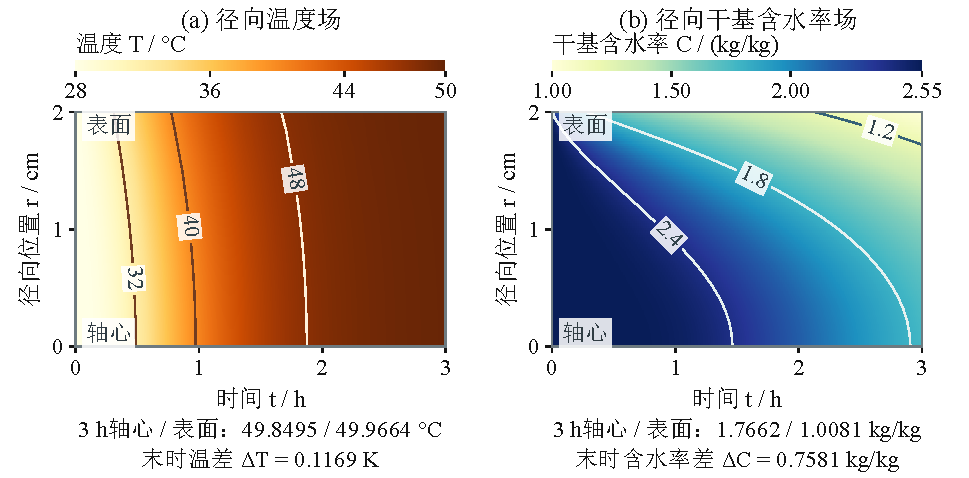
\includegraphics[width=0.94\textwidth]{figures/legibility_q2/q2_fields.pdf}
\caption{第二问前3小时径向温度场与干基含水率场的时空演化。横轴为时间，纵轴为径向位置，颜色表示场量大小；等值线辅助辨识时空分布，末时径向差值另作标注。}
\label{fig:q2-profiles}
\end{figure}

图\ref{fig:q2-profiles}左图显示温度总体随时间升高，并逐渐趋于径向均匀；
右图显示含水率先在表层下降，低含水区域随后向内部扩展，径向差异仍较明显。

第二问$0.5\unit{h}$轴心温度32.1892\celsius，低于第一问同一
时刻；这是从初态使用不同物性、尤其初始有效热容量更大的正常结果，
不是问间接口错误。第一问和第二问是不同参数情形，不能共用一段预热轨迹。

\subsection{升温促进与失水抑制的竞争}
将附录3扩散系数相对初态取对数，可精确分解为
\begin{equation}
\begin{aligned}
\ln\frac{D(t,r)}{D_0}&=H(t,r)+M(t,r),\\
H&=3850\left(\frac1{301.15}-\frac1{T_K}\right),\qquad
M=0.45\left(\frac1{2.55}-\frac1C\right).
\end{aligned}
\label{eq:q2-log-mechanism}
\end{equation}
其中$D_0=5.64168037\times10^{-9}\unit{m^2/s}$。
$H$度量沿当前轨迹的累计温度贡献，$M$度量累计含水率贡献；这是代数
分解，不能当作独立改变某一因素的因果贡献百分比。

图\ref{fig:q2-mechanism}展示上述分解；前$3\unit{h}$逐秒采样中，轴心与表面扩散率
分别于约$2.46\unit{h}$和$2.02\unit{h}$达到该时段的采样峰值，随后回落。

\begin{figure}[htbp]
\centering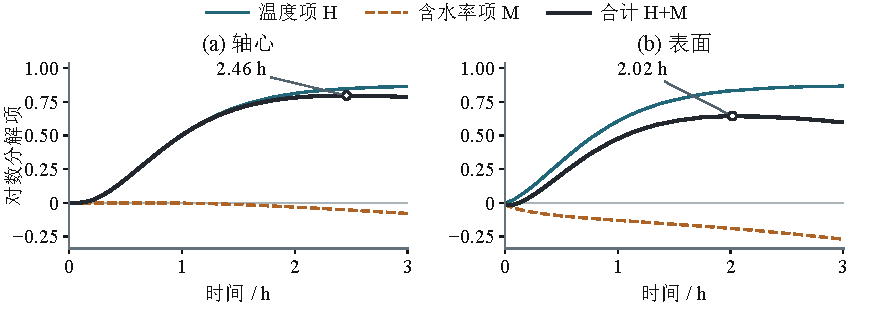
\includegraphics[width=\linewidth]{figures/legibility_q2/q2_mechanism.pdf}
\caption{第二问前3小时轴心与表面的扩散率对数分解。$H$为温度贡献，$M$为含水率贡献，$H+M=\ln(D/D_0)$；标记为逐秒采样峰值，不表示连续时间严格极值。}
\label{fig:q2-mechanism}
\end{figure}

$3\unit{h}$时，轴心与表面的$D/D_0$分别为2.1957与1.8207，说明相对
初态累计升温促进仍占优势；但最后半小时，两处扩散率分别下降约1.06\%
和3.16\%。因此“扩散系数全程单调增加”不成立。表面还曾在早期每秒
采样的第144秒达到$D/D_0=0.983282$的局部最低值。温度变化和失水抑制
的竞争随阶段变化，前3小时的累计主导关系不能直接用于判定末期干燥瓶颈。

在同一320区间有限体积网格上单独扰动交换系数，$h_m$降低、提高20\%
时，$3\unit{h}$表面含水率分别为1.1775、0.8737；相应轴心值为1.8581、
1.6921。对这一输出和扰动区间，水分交换系数的影响明显大于数值误差。
该对照为人为情景而非参数置信区间（见第\ref{sec:environment-scenarios}节），
不能替代气固水分基准识别\cite{dasilva2014,adrover2020}。

\subsection{独立验证与适用范围}
以下核查数值输出与模型账本的一致性，并检验降维适用范围。

前3小时已有节点有限体积逐级加密至2560区间及Richardson外推，
另用独立空间离散与Radau积分核对。全程轨迹与该外推轨迹在前3小时
共同采样点的最大温差约$1.07\times10^{-9}\unit{K}$、含水率差约
$8.41\times10^{-8}\unit{kg/kg}$；前3小时温湿表及规定60个论文表值四位一致。
有限体积外推是这一前3小时交叉验证的来源，不是完整工作簿的生成方法。

长时段另与已完成的160阶BDF轨迹在全部60秒采样点及同一执行端点比较，
最大温湿差约$3.27\times10^{-9}\unit{K}$与$9.33\times10^{-9}\unit{kg/kg}$，
四位输出一致。当前869万余格工作簿与同源未舍入轨迹的舍入核对全部通过，
该检查支持导出一致性；高阶独立参考覆盖的是所列采样点，不能把导出
一致性误写成全部逐秒状态均另作了独立求解。

原有限体积有效水分账本的最大残差约$6.51\times10^{-12}\unit{kg/kg}$。
热账本核对的是有效热容量积分与边界热流，即比较
$\int\!\int S(C)T_t\,\mathrm dV\mathrm dt$与累计边界热量，
相对残差约$3.11\times10^{-11}$，并非$\int ST\,\mathrm dV$的末初差，
更不构成潜热、携焓及真实总能量已经闭合的证明。
同物理$80\times256$二维配对在前3小时已检查采样点的中截面最大温湿差
约为$1.692\times10^{-3}\unit{K}$、$2.247\times10^{-5}\unit{kg/kg}$。
这支持中截面的工程近似，但不能保证降维后所有四位显示相同；长期全域
达标须结合第三问终点证据，不能直接沿用前3小时的几何误差。
本问早期大通量阶段亦受相变能量缺口约束，相关量级诊断与闭合限制见第\ref{sec:limitations}节。

综上，温湿场响应不同步，升温促进与失水抑制呈阶段性竞争；
所得同一条轨迹为问题三追踪径向最大含水率、判定干燥终点提供计算基础。
\FloatBarrier
\endgroup
